\documentclass[11pt,a4paper]{article}

\usepackage[T1]{fontenc}
\usepackage{lmodern}
\usepackage[margin=2.5cm]{geometry}
\usepackage{amsmath,amssymb,mathtools}
\usepackage{booktabs}
\usepackage{array}
\usepackage{graphicx}
\usepackage{xcolor}
\usepackage{microtype}
\usepackage{enumitem}
\usepackage[font=small,labelfont=bf]{caption}
\usepackage{tikz}
\usetikzlibrary{arrows.meta,positioning,fit,backgrounds}
\usepackage[numbers,sort&compress]{natbib}
\usepackage[colorlinks=true,linkcolor=blue!50!black,citecolor=blue!50!black,urlcolor=blue!50!black]{hyperref}
\usepackage[capitalise,noabbrev]{cleveref}
\hypersetup{pdftitle={A Real-Time Crypto Market Data Pipeline with Honest Latency and Loss Monitoring},
  pdfauthor={Kevin Feltrin},
  pdfkeywords={market data, websocket, TimescaleDB, latency, clock synchronisation, monitoring}}

% Generated by analysis/make_figures.py -- do not edit by hand.
\newcommand{\TestCount}{50}
\newcommand{\BusiestTradesPerS}{357}
\newcommand{\CapacityRatio}{33}
\newcommand{\TotalTradesText}{1\,253\,736}
\newcommand{\TotalLive}{926\,623}
\newcommand{\TotalRecoveredTrades}{327\,113}
\newcommand{\BaselineMinutes}{100}
\newcommand{\ChaosMinutes}{37}
\newcommand{\StopMinutes}{5.1}
\newcommand{\TotalHours}{2.4}
\newcommand{\ExperimentDate}{24 November 2026}
\newcommand{\ExperimentStart}{13:33}
\newcommand{\ExperimentEnd}{15:54}
\newcommand{\QuietMinutes}{58}
\newcommand{\NoisyMinutes}{16}
\newcommand{\QuietOffsetMs}{\ensuremath{-1021}}
\newcommand{\QuietOffsetRangeMs}{\ensuremath{-1024} to \ensuremath{-1019}}
\newcommand{\QuietOffsetUncMs}{2.9}
\newcommand{\LatBinancePfifty}{119}
\newcommand{\LatBinancePninetynine}{379}
\newcommand{\LatBinanceMin}{111.9}
\newcommand{\RttBinanceHalf}{198}
\newcommand{\LatCoinbasePfifty}{57}
\newcommand{\LatCoinbasePninetynine}{221}
\newcommand{\LatCoinbaseMin}{44.7}
\newcommand{\RttCoinbaseHalf}{44}
\newcommand{\LatKrakenPfifty}{15}
\newcommand{\LatKrakenPninetynine}{63}
\newcommand{\LatKrakenMin}{8.9}
\newcommand{\RttKrakenHalf}{10}
\newcommand{\ClockDriftMsPerHour}{1.9}
\newcommand{\ClockDriftPpm}{0.5}
\newcommand{\NtpSamples}{211}
\newcommand{\NtpDelayMedianMs}{10.4}
\newcommand{\NtpBestOffsetMedianMs}{\ensuremath{-1018.9}}
\newcommand{\NtpBestOffsetMinMs}{\ensuremath{-1024.5}}
\newcommand{\NtpBestOffsetMaxMs}{\ensuremath{-1014.9}}
\newcommand{\NtpOffsetMinMs}{\ensuremath{-1035}}
\newcommand{\NtpOffsetMaxMs}{\ensuremath{-908}}
\newcommand{\NtpDelayMaxMs}{243}
\newcommand{\BinanceRestOffsetMs}{\ensuremath{-1001}}
\newcommand{\BinanceRestUncMs}{132}
\newcommand{\ProbeQuietSeconds}{3\,502}
\newcommand{\ProbeQuietDiffMedianMs}{0.8}
\newcommand{\ProbeQuietDiffPninetynineMs}{221}
\newcommand{\ProbeQuietPipeOverHalfSec}{20}
\newcommand{\ProbeQuietProbeOverHalfSec}{12}
\newcommand{\ProbeQuietCorr}{0.28}
\newcommand{\ProbeNoisySeconds}{947}
\newcommand{\ProbeNoisyDiffMedianMs}{1.1}
\newcommand{\ProbeNoisyDiffPninetynineMs}{31}
\newcommand{\ProbeNoisyPipeOverHalfSec}{0}
\newcommand{\ProbeNoisyProbeOverHalfSec}{3}
\newcommand{\ProbeNoisyCorr}{0.39}
\newcommand{\ProbeMedianMs}{116.7}
\newcommand{\PipelineMedianMs}{117.8}
\newcommand{\ProbeMaxMs}{595502}
\newcommand{\EminusTMedianMs}{0.34}
\newcommand{\EminusTMaxMs}{97}
\newcommand{\TotalMissing}{391\,457}
\newcommand{\TotalRecovered}{391\,457}
\newcommand{\RecoveredPctText}{100\%}
\newcommand{\ChaosDisconnects}{12}
\newcommand{\BookResyncs}{6}
\newcommand{\InSessionGaps}{0}
\newcommand{\UnrecoveredTotal}{0}
\newcommand{\BaselineDisconnects}{0}
\newcommand{\BaselineDisconnectReasons}{none}
\newcommand{\ChaosDowntimeMedianS}{11.7}
\newcommand{\ChaosDowntimeTotalS}{1649}
\newcommand{\RepairMedianS}{3.1}
\newcommand{\RepairMaxS}{160}
\newcommand{\LargestGap}{120\,213}
\newcommand{\LargestGapWhere}{Binance BTC-USDT}
\newcommand{\RestartMissing}{65\,224}
\newcommand{\SuspensionMinutes}{26}
\newcommand{\SuspensionStart}{15:23}
\newcommand{\SuspensionMissing}{319\,295}
\newcommand{\SuspensionRecovered}{319\,295}
\newcommand{\FailedAttempts}{21}
\newcommand{\QuotesStored}{115\,084}
\newcommand{\CrossedQuotes}{0}
\newcommand{\AuditReference}{1\,216\,302}
\newcommand{\AuditMissing}{0}
\newcommand{\AuditMismatched}{0}
\newcommand{\AuditUnexpected}{0}
\newcommand{\AuditRecovered}{325\,778}
\newcommand{\IngestQuietPfifty}{125}
\newcommand{\IngestQuietPninetynine}{318}
\newcommand{\LoopLagQuietPninetynine}{24.2}
\newcommand{\DbWriteQuietPninetynine}{93.4}
\newcommand{\IngestNoisyPfifty}{126}
\newcommand{\IngestNoisyPninetynine}{298}
\newcommand{\LoopLagNoisyPninetynine}{24.1}
\newcommand{\DbWriteNoisyPninetynine}{97.3}
\newcommand{\IngestChaosPfifty}{132}
\newcommand{\IngestChaosPninetynine}{422}
\newcommand{\LoopLagChaosPninetynine}{24.7}
\newcommand{\DbWriteChaosPninetynine}{115}
\newcommand{\ParseBinancePfiftyUs}{23}
\newcommand{\BatchRowsQuietPfifty}{6.4}
\newcommand{\TradesRows}{1\,318\,080}
\newcommand{\TradesMBUncompressed}{348}
\newcommand{\TradesMBCompressed}{17.1}
\newcommand{\CompressionRatio}{20.3}
\newcommand{\BytesPerTradeCompressed}{14}
\newcommand{\BenchBestRowsPerS}{11\,646}
\newcommand{\BenchSpeedupMax}{3.7}


\newcommand{\code}[1]{\texttt{#1}}
\newcommand{\repo}{\url{https://github.com/KvnFltr/crypto-market-data-pipeline}}
\newcommand{\ms}{\,ms}

\title{\textbf{A Real-Time Crypto Market Data Pipeline}\\[4pt]
  \large with Honest Latency and Loss Monitoring}
\author{Kevin Feltrin}
\date{November 2026}

\begin{document}
\maketitle

\begin{abstract}
\noindent
Every quantitative strategy starts with market data, and two questions about that data are rarely answered
with numbers: how late is it, and is any of it missing? This report describes \code{marketpipe}, a pipeline
that ingests trades and order book updates from three crypto exchanges (Binance, Coinbase, Kraken) over
websockets, stores them in TimescaleDB, and measures both quantities. Losses are counted exactly by checking
the venues' sequence numbers, and every gap is repaired from the venues' REST history; storage is idempotent,
so the result is effectively-once. Latencies are corrected for the offset of the local clock, measured against
NTP servers, and reported with the uncertainty of that correction. In a live experiment of \TotalHours{} hours
(\TradesRows{} trades) with a planned restart, \ChaosDisconnects{} injected disconnections and an unplanned
\SuspensionMinutes-minute suspension of the host, the pipeline detected \TotalMissing{} missing trades and
recovered \RecoveredPctText{} of them; an independent audit against each venue's history found \AuditMissing{}
missing and \AuditMismatched{} altered trades out of \AuditReference. The local clock turned out to be one second
ahead of UTC: uncorrected, every latency would have been overstated by a second. Corrected, the median latency
from Paris is \LatBinancePfifty\ms{} for Binance (Tokyo), \LatCoinbasePfifty\ms{} for Coinbase and
\LatKrakenPfifty\ms{} for Kraken. A control experiment with an independent receiver shows that the pipeline adds
about a millisecond to the median and that most latency spikes originate upstream. Code, tests, dashboards and
data are available at \repo.
\end{abstract}

\tableofcontents
\bigskip

% =====================================================================================================
\section{Introduction}

A market data pipeline is judged on two properties that are easy to claim and hard to verify. The first is
\emph{completeness}: a strategy back-tested on data with silent holes, or trading on a feed that dropped the
last two seconds, is wrong in ways that do not show up until it loses money. The second is \emph{timeliness}:
an estimate of latency that ignores the error of the local clock, or that averages away the tail, says little
about the delay a strategy will actually experience \citep{tene2015}.

This project builds a small pipeline that takes both seriously:
\begin{itemize}[nosep]
  \item it never drops data silently: every message carries a venue sequence number, so a loss is a measured
        quantity, and every lost trade is recovered from the venue's REST history;
  \item it measures latency against a corrected clock and reports the uncertainty of that correction, its own
        contribution separately, and the physical lower bound set by the speed of light;
  \item it exposes all of this as metrics, dashboards and alerts, and checks its own completeness with an
        independent audit.
\end{itemize}
\Cref{sec:architecture} presents the architecture, \cref{sec:venues} the venues and their sequencing guarantees,
\cref{sec:losses,sec:latency} the treatment of losses and latency, \cref{sec:storage,sec:monitoring,sec:testing}
storage, monitoring and testing. \Cref{sec:results} reports a live experiment.

% =====================================================================================================
\section{Architecture}\label{sec:architecture}

\begin{figure}[ht]
\centering
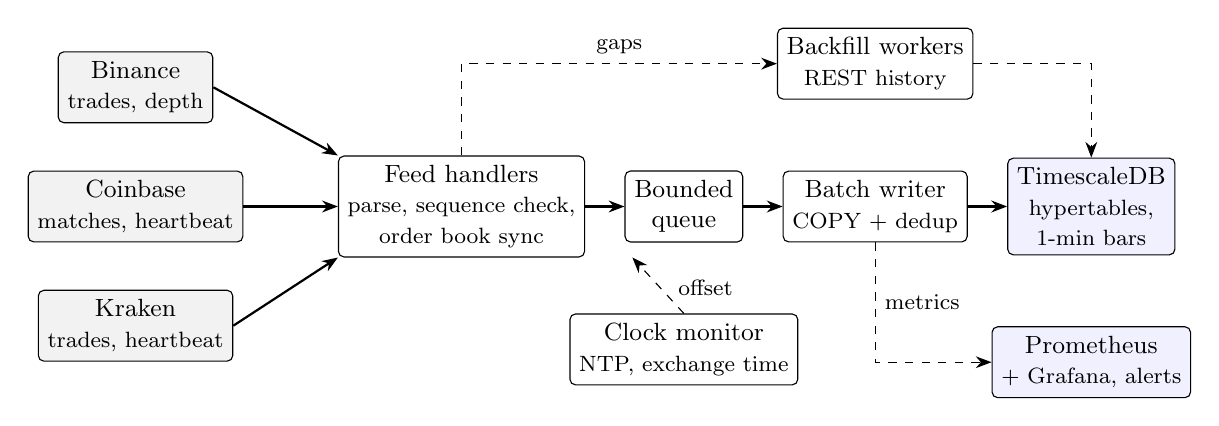
\begin{tikzpicture}[
  node distance=6mm and 5mm, font=\small,
  box/.style={draw, rounded corners=2pt, align=center, minimum height=9mm, fill=white},
  ext/.style={box, fill=gray!10},
  store/.style={box, fill=blue!6},
  arr/.style={-{Stealth[length=2mm]}, thick},
  side/.style={-{Stealth[length=2mm]}, dashed}]
  \node[ext] (bn) {Binance\\ \footnotesize trades, depth};
  \node[ext, below=of bn] (cb) {Coinbase\\ \footnotesize matches, heartbeat};
  \node[ext, below=of cb] (kr) {Kraken\\ \footnotesize trades, heartbeat};
  \node[box, right=12mm of cb, minimum width=30mm] (feed) {Feed handlers\\ \footnotesize parse, sequence check,\\ \footnotesize order book sync};
  \node[box, right=of feed] (queue) {Bounded\\ queue};
  \node[box, right=of queue] (writer) {Batch writer\\ \footnotesize COPY + dedup};
  \node[store, right=of writer] (db) {TimescaleDB\\ \footnotesize hypertables,\\ \footnotesize 1-min bars};
  \node[box, above=9mm of writer] (backfill) {Backfill workers\\ \footnotesize REST history};
  \node[box, below=9mm of queue] (clock) {Clock monitor\\ \footnotesize NTP, exchange time};
  \node[store, below=9mm of db] (prom) {Prometheus\\ \footnotesize + Grafana, alerts};
  \draw[arr] (bn.east) -- (feed.north west);
  \draw[arr] (cb.east) -- (feed.west);
  \draw[arr] (kr.east) -- (feed.south west);
  \draw[arr] (feed) -- (queue);
  \draw[arr] (queue) -- (writer);
  \draw[arr] (writer) -- (db);
  \draw[side] (feed.north) |- node[pos=0.75, above, font=\footnotesize] {gaps} (backfill.west);
  \draw[side] (backfill.east) -| (db.north);
  \draw[side] (clock.north) -- node[pos=0.45, right=1mm, font=\footnotesize] {offset} ([xshift=6mm]feed.south east);
  \draw[side] (writer.south) |- node[pos=0.25, right, font=\footnotesize] {metrics} (prom.west);
\end{tikzpicture}
\caption{Data flow. Solid arrows carry market data (websockets from the venues); dashed arrows carry gaps, clock corrections and metrics.}
\label{fig:architecture}
\end{figure}

The pipeline (\cref{fig:architecture}) is a single Python process built on \code{asyncio}. One feed handler per
venue owns a websocket connection: it decodes each message into normalised events (trades, depth updates,
heartbeats), checks sequence numbers, maintains the Binance order books, and puts trades and best quotes on a
bounded queue. A batch writer drains the queue into TimescaleDB. Gaps are handed to one backfill worker per
venue, which fetches the missing trades over REST and stores them through the same idempotent path. A clock
monitor samples NTP servers and the Binance server clock. All components export Prometheus metrics.

\paragraph{Why one event loop.} At the rates involved (hundreds of messages per second, a few thousand during
bursts) the work per message is a few tens of microseconds, so one core is ample and a single event loop avoids
any synchronisation. The design choice that matters is \emph{where} delay can accumulate: reads, writes and REST
calls are all non-blocking, and the only shared resource, the queue, is bounded. When the database falls behind,
\code{queue.put} blocks the readers; the exchange eventually disconnects the slow consumer, and the resulting gap
is repaired like any other. Nothing is ever dropped to keep up. On Linux the loop runs on \code{uvloop}.

% =====================================================================================================
\section{Venues and sequencing guarantees}\label{sec:venues}

Exact loss accounting relies on what each venue guarantees about its message numbering
(\cref{tab:venues}). All three number their trades with an integer that increases by exactly one per trade and
per instrument, and all three publish their trade history over REST, which makes every lost trade recoverable.

\begin{table}[ht]
\centering
\caption{Feeds used, with their sequencing and recovery semantics.}
\label{tab:venues}
\small
\begin{tabular}{@{}>{\raggedright\arraybackslash}p{1.5cm}>{\raggedright\arraybackslash}p{2.6cm}>{\raggedright\arraybackslash}p{3.3cm}>{\raggedright\arraybackslash}p{3.2cm}>{\raggedright\arraybackslash}p{3.0cm}@{}}
\toprule
Venue & Stream & Sequence & Timestamps & Recovery \\
\midrule
Binance & \code{@trade} & trade id \code{t}, $+1$ per trade & trade time $T$ and event time $E$, $\mu$s & \code{historicalTrades} by id \\
        & \code{@depth@100ms} & update ids $[U,u]$, chained & event time, $\mu$s & none: resync from snapshot \\
Coinbase & \code{matches} & \code{trade\_id}, $+1$ per trade & trade time, $\mu$s & \code{/trades} by id, backwards \\
         & \code{heartbeat} & last trade id, every second & -- & reveals silent losses \\
Kraken & \code{trade} (API v2) & \code{trade\_id}, $+1$ per trade & trade time, $\mu$s & \code{/Trades} by time \\
\bottomrule
\end{tabular}
\end{table}

Several details matter for correctness. The aggressor side is reported differently: Binance gives a
``buyer is maker'' flag, Coinbase the side of the \emph{maker} order, Kraken the side of the taker; the adapters
normalise all three to the aggressor side. Binance closes connections after 24 hours, so the pipeline rotates
them after 23. Kraken's REST history is indexed by time rather than by trade id, so recovery starts searching at
the exchange time of the last trade received before the gap.

% =====================================================================================================
\section{Detecting and recovering lost messages}\label{sec:losses}

\subsection{Gap detection}

A websocket runs over TCP, so within one connection the network cannot reorder or drop messages. Losses still
happen: venues drop messages for slow consumers, and every message published while we are disconnected is
lost. For each instrument the feed handler compares the trade id $s_n$ with the last one seen, $s_{n-1}$:
\[
  s_n = s_{n-1} + 1 \;\Rightarrow\; \text{in order}, \quad
  s_n \le s_{n-1} \;\Rightarrow\; \text{duplicate}, \quad
  s_n > s_{n-1} + 1 \;\Rightarrow\; \text{gap } [s_{n-1}+1,\, s_n-1].
\]
Each gap is classified by cause: \emph{in session} (no reconnection in between), \emph{reconnect} (first trade
after a reconnection), \emph{restart} (first trade after the process started, compared with the last trade
stored in the database), or \emph{heartbeat}. The last case covers a quiet market: Coinbase announces in its
heartbeat the id of the last trade, and an announced id that never arrives reveals a loss that no subsequent
trade would expose. Because a heartbeat may overtake the trades it announces, it is only acted upon after a
two-second grace period.

A connection can also fail silently: a half-open TCP connection stays ``up'' while nothing arrives. Every feed
therefore has a staleness deadline (15 to 30 seconds without any message, heartbeats included) after which it
reconnects. Reconnections use exponential backoff with full jitter, so that many clients do not retry in
lockstep \citep{brooker2015}.

\subsection{Recovery and effectively-once storage}

Every gap is stored in a \code{gaps} table, then repaired by a backfill worker that downloads the missing trades
from the venue's REST history and stores them with \code{source = 'rest'}. The outcome is recorded:
\emph{recovered}, \emph{partial} or \emph{unrecoverable}. Delivery from the venues is therefore at least once
(a trade may arrive twice: live, and again from the history), and the storage layer makes it effectively once
by deduplicating on the trade id (\cref{sec:storage}). The same mechanism covers process restarts: at start-up
each feed is seeded with the last trade id stored, so that the trades published while the pipeline was down
form an ordinary gap.

\subsection{Order books}

Binance depth updates cover ranges of book update ids $[U,u]$ that must chain: $U_{n} = u_{n-1}+1$. They are
applied to a local book built from a REST snapshot, following the venue's procedure \citep{binance-ws}: buffer
the stream, fetch a snapshot with id $L$, drop updates with $u \le L$, require the first remaining update to
satisfy $U \le L+1 \le u$, then apply updates in order. A broken chain cannot be repaired by replaying
updates, so it triggers a rebuild from a new snapshot and is recorded as a \emph{resynced} gap. In practice the
snapshot is often \emph{ahead} of the stream; the synchroniser then keeps it and waits for the stream to catch
up instead of fetching a new one, which brought the time to a live book from about 15 seconds to under one.
The best bid and offer are stored whenever they change.

% =====================================================================================================
\section{Measuring latency honestly}\label{sec:latency}

\subsection{Definitions}

For a trade stamped $t_{\mathrm{ex}}$ by the venue and received at local wall-clock time $t_{\mathrm{rx}}$, the
\emph{exchange latency} is $L = t_{\mathrm{rx}} - t_{\mathrm{ex}}$. It compares two clocks. If the local clock
differs from true time by $\varepsilon$, the measured value is off by exactly $\varepsilon$, which can reach a
second on a desktop machine, as it did in our experiment. The pipeline therefore estimates the offset $\theta = -\varepsilon$ of the
local clock against reference clocks and reports $L = t_{\mathrm{rx}} + \theta - t_{\mathrm{ex}}$, assuming
that the venues' clocks are synchronised to UTC.

\subsection{Clock offset and its uncertainty}

The offset is measured with SNTP \citep{rfc4330,mills1991}. A request leaves at local time $t_0$, the server
stamps its reception $t_1$ and its reply $t_2$, and the reply arrives at $t_3$. Then
\[
  \hat\theta = \frac{(t_1 - t_0) + (t_2 - t_3)}{2}, \qquad \delta = (t_3 - t_0) - (t_2 - t_1),
\]
and, whatever the split of the round-trip delay $\delta$ between the two directions, the true offset lies within
$\hat\theta \pm \delta/2$. Like NTP's clock filter, the pipeline keeps the last samples and uses the one with
the smallest delay. As a cross-check it applies Cristian's algorithm \citep{cristian1989} to Binance's server
time, $\hat\theta = T_{\mathrm{server}} - (t_0+t_3)/2$, with uncertainty $\pm (t_3 - t_0)/2$. Raw receipt times
are stored unchanged; the correction is applied at analysis time from the recorded clock samples.

\subsection{What else is in the number}

Three other effects are bounded explicitly.
\begin{enumerate}[nosep]
  \item \emph{Venue-side delay.} Binance publishes both the trade time $T$ and the event time $E$ at which the
        message was emitted, which splits $L$ into an internal part $E - T$ and a transport part
        $t_{\mathrm{rx}} - E$, each measured on a single clock domain except for the offset.
  \item \emph{Our own delay.} $t_{\mathrm{rx}}$ is taken when the event loop hands the message to the feed
        handler, so a busy loop inflates it. The pipeline measures the scheduling lag of its event loop
        continuously, and its internal latencies (receipt to database commit) on the monotonic clock.
  \item \emph{Physics.} Light in fibre travels at about $2\times10^5$ km/s. Paris is 9\,712 km from Tokyo, where
        Binance's spot matching engine is publicly reported to run (AWS \code{ap-northeast-1}), and 6\,186 km
        from northern Virginia (AWS \code{us-east-1}, reported for Coinbase), so one-way latencies below 48.6\ms{}
        and 30.9\ms{} respectively are impossible; real routes are longer.
\end{enumerate}
Finally, a \emph{control experiment} separates the pipeline from the outside world: a minimal process that does
nothing but receive the Binance trade stream records the same latency in parallel (\cref{sec:res-latency}).

% =====================================================================================================
\section{Storage}\label{sec:storage}

Trades and quotes are stored in TimescaleDB hypertables partitioned by exchange time in one-day chunks
\citep{timescale}. Writes are batched: a batch is flushed after 2\,000 rows or 100\ms, whichever comes first,
which bounds the delay added by batching. A batch is copied with \code{COPY} into a temporary table and inserted
into the hypertable with a single statement that skips trades already stored:
\begin{verbatim}
INSERT INTO trades
SELECT DISTINCT ON (venue, symbol, trade_id) ... FROM trades_stage s
WHERE NOT EXISTS (
    SELECT 1 FROM trades t
    WHERE (t.venue, t.symbol, t.trade_id) = (s.venue, s.symbol, s.trade_id)
      AND t.exchange_ts BETWEEN s.exchange_ts - '1 min'
                            AND s.exchange_ts + '1 min')
ON CONFLICT DO NOTHING
\end{verbatim}
Two details are worth noting. A unique constraint on a hypertable must include the partitioning column, so the
primary key is (venue, symbol, trade\_id, exchange\_ts); but the live and REST copies of a trade can carry
timestamps rounded differently by a microsecond, so deduplication matches trade ids within a one-minute window,
which keeps the lookup on recent chunks. Within a batch, the live copy is preferred because it carries the
receipt time. A continuous aggregate maintains one-minute OHLCV bars, and chunks older than a day are compressed
into columnar form.

% =====================================================================================================
\section{Monitoring}\label{sec:monitoring}

The pipeline exports Prometheus metrics: messages and bytes per venue; latency histograms (exchange to receipt,
receipt to commit, parse time, event-loop lag, websocket ping round trip); gaps, missing, recovered and
unrecovered trades by venue and cause; reconnections by reason; order book resyncs; queue depth; batch sizes,
write times and errors; clock offset and delay. A provisioned Grafana dashboard combines them with queries on
TimescaleDB (prices, trades per minute, latest gaps, disconnections as annotations), and alert rules cover the
failure modes that matter (\cref{tab:alerts}). The rules follow the usual site-reliability practice of alerting
on symptoms that need a human \citep{beyer2016}: an unrecoverable loss pages; a recovered gap does not.

\begin{table}[ht]
\centering
\caption{Prometheus alert rules.}
\label{tab:alerts}
\small
\begin{tabular}{@{}lll@{}}
\toprule
Alert & Condition & Severity \\
\midrule
FeedStale & no message for 30 s, sustained 1 min & critical \\
FeedDisconnected & websocket down for 2 min & critical \\
TradesLost & any unrecoverable trade in 15 min & critical \\
DatabaseWriteErrors & any failed batch write in 5 min & critical \\
GapRateHigh & more than 5 trade gaps in 10 min & warning \\
ExchangeLatencyHigh & p99 above 1 s for 5 min & warning \\
WriterBacklog & more than 50\,000 queued events for 1 min & warning \\
ClockOffsetLarge & local clock more than 50\ms{} from NTP for 10 min & warning \\
\bottomrule
\end{tabular}
\end{table}

% =====================================================================================================
\section{Testing}\label{sec:testing}

The test suite (\TestCount{} tests, run in continuous integration on Python 3.11 to 3.13 against a TimescaleDB
service container) has three layers.
\begin{itemize}[nosep]
  \item \emph{Unit tests}: sequence tracking, SNTP encoding and offset arithmetic (including a local NTP server
        whose clock is 50\ms{} ahead), the parsers on messages captured from the live feeds, REST pagination of
        each venue, the order book procedure (snapshot ahead of the stream, broken chain, resync), backoff.
  \item \emph{A fake exchange}: a local websocket server that produces a trade tape whether or not anyone is
        listening, and can silently drop messages, cut connections and refuse reconnections. Feed tests check
        that every trade of the tape is either received or covered by a detected gap.
  \item \emph{End-to-end tests} on a real database: the full pipeline runs against the fake exchange with
        dropped messages, cut connections, random forced disconnections and a restart, and the database must
        hold every trade of the tape exactly once. The completeness audit must find a trade deleted by hand
        and a price altered by hand.
\end{itemize}
Linting (\code{ruff}) and static typing (\code{mypy --strict}) are enforced in CI, and the Docker image is built
and smoke-tested.

% =====================================================================================================
\section{Experiment and results}\label{sec:results}

% Results of the live experiment. Numbers come from generated/results.tex (analysis/make_figures.py).

\subsection{Setup}

The pipeline ran on a laptop in Paris (Intel Core i7-1260P, 16 hardware threads, Windows 11) connected to a
university Wi-Fi network, with TimescaleDB, Prometheus and Grafana in Docker, on \ExperimentDate{} from
\ExperimentStart{} to \ExperimentEnd{} UTC. It followed BTC and ETH on Binance (trades and order books),
Coinbase and Kraken (trades). The experiment had three phases:
\begin{enumerate}[nosep]
  \item a \emph{baseline} run of \BaselineMinutes{} minutes, including a planned \emph{noisy-neighbour} phase of
        \NoisyMinutes{} minutes during which the test suite and a storage benchmark ran in a loop on the same
        machine, competing for CPU and for the database;
  \item a \emph{planned stop} of \StopMinutes{} minutes, to test recovery after a restart;
  \item a \emph{fault-injection} run, during which each feed was forcibly disconnected at exponentially
        distributed intervals (mean 2 minutes) and kept down for 1 to 20 seconds.
\end{enumerate}
The independent latency probe ran throughout. Two earlier attempts are worth mentioning because they shaped the
setup: the first was interrupted when the laptop went to sleep, and the second failed because the university
network filters port 9443, on which Binance's streams are usually documented; the pipeline now connects on
port 443. \Cref{tab:runs} summarises the data collected and \cref{fig:throughput} the activity of each venue.

\begin{table}[ht]
\centering
\caption{Trades stored per run, by exchange time. Recovered trades were missed by the websocket and fetched
from the venue's history.}
\label{tab:runs}
\small
% Generated by analysis/make_figures.py
\begin{tabular}{llrrr}
\toprule
Run & Venue & Trades stored & live & recovered \\
\midrule
baseline & Binance & 653\,619 & 653\,146 & 473 \\
 & Coinbase & 203\,373 & 203\,265 & 108 \\
 & Kraken & 16\,342 & 16\,342 & 0 \\
\midrule
chaos & Binance & 277\,634 & 39\,253 & 238\,381 \\
 & Coinbase & 94\,827 & 13\,462 & 81\,365 \\
 & Kraken & 7\,941 & 1\,155 & 6\,786 \\
\bottomrule
\end{tabular}

\end{table}

\begin{figure}[ht]
  \centering
  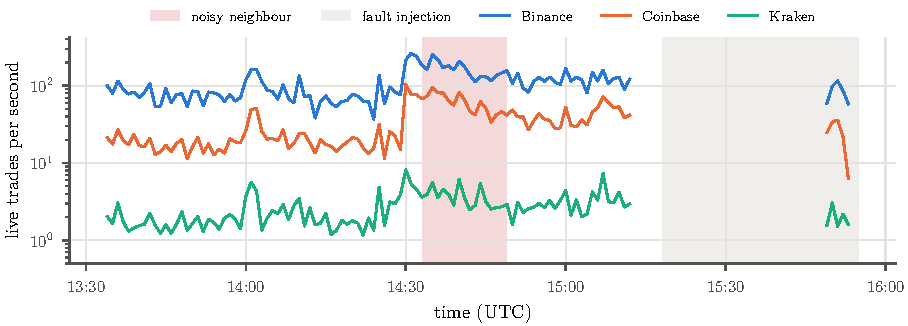
\includegraphics[width=\textwidth]{figures/throughput.pdf}
  \caption{Trades received live per second, per minute and venue (logarithmic scale). Shaded: the
  noisy-neighbour phase (red) and the fault-injection run (grey). The fault-injection run is interrupted by a
  26-minute suspension of the host, discussed in \cref{sec:res-losses}.}
  \label{fig:throughput}
\end{figure}

\subsection{Latency}\label{sec:res-latency}

\paragraph{Clock.} The first finding is about the local clock: during the whole experiment it was about
\emph{one second} ahead of UTC (\cref{fig:clock}). Over \NtpSamples{} NTP samples with a median round-trip
delay of \NtpDelayMedianMs\ms{}, the best samples put the offset between \NtpBestOffsetMinMs{} and
\NtpBestOffsetMaxMs\ms, drifting by \ClockDriftMsPerHour\ms{} per hour (\ClockDriftPpm{} ppm). Cristian's
algorithm on Binance's server time gives \BinanceRestOffsetMs\ms{} $\pm$ \BinanceRestUncMs\ms: an independent
confirmation, two orders of magnitude less precise because of the round trip to Tokyo. Without the
correction, every latency in this report would be overstated by a second, making Binance look ten times
slower than it is. The operating system's own synchronisation had not corrected this offset, which is common
on machines that synchronise rarely. Latencies below are corrected minute by minute; the uncertainty of the
correction over the quiet baseline is about $\pm$\QuietOffsetUncMs\ms.

\begin{figure}[ht]
  \centering
  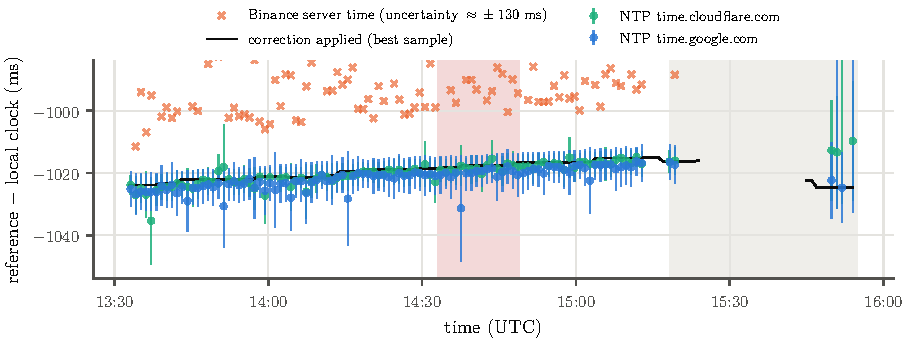
\includegraphics[width=\textwidth]{figures/clock.pdf}
  \caption{Offset of the local clock against two NTP servers (error bars: $\pm\delta/2$) and Binance's server
  time, and the correction applied to latencies.}
  \label{fig:clock}
\end{figure}

\paragraph{Exchange to receipt.} \Cref{tab:latency,fig:latency-cdf} give the distribution of the corrected
latency over the quiet part of the baseline (\QuietMinutes{} minutes). The minima are consistent with
geography: \LatBinanceMin\ms{} to Binance against a fibre bound of 48.6\ms{} (real routes to Tokyo are much
longer than the great circle), \LatCoinbaseMin\ms{} to Coinbase against 30.9\ms{}. Kraken, at
\LatKrakenMin\ms, is evidently served from much closer, presumably a European point of presence. The last
column, half the median round trip of websocket pings, estimates the one-way network delay without any clock.
It matches the latency minima for Coinbase (\RttCoinbaseHalf{} against \LatCoinbaseMin\ms) and Kraken
(\RttKrakenHalf{} against \LatKrakenMin\ms), which is a check of the clock correction itself. Binance answers
pings much more slowly than it streams data (\RttBinanceHalf\ms), so a ping-based estimate would be wrong there.

\begin{table}[ht]
\centering
\caption{Exchange time to receipt (ms), corrected for the local clock (about \QuietOffsetMs\ms), over the quiet
baseline, and half the median websocket ping round trip.}
\label{tab:latency}
\small
% Generated by analysis/make_figures.py
\begin{tabular}{lrrrrrrrrr}
\toprule
Venue & Trades & min & p1 & p50 & p90 & p99 & p99.9 & max & ping RTT/2 \\
\midrule
Binance & 309\,280 & 111.9 & 114.4 & 119.3 & 136.4 & 379 & 683 & 1675 & 198.3 \\
Coinbase & 81\,178 & 44.7 & 47.1 & 57.0 & 107.4 & 221 & 300 & 515 & 44.4 \\
Kraken & 7\,858 & 8.9 & 10.2 & 15.2 & 26.4 & 63 & 168 & 1189 & 9.6 \\
\bottomrule
\end{tabular}

\end{table}

\begin{figure}[ht]
  \centering
  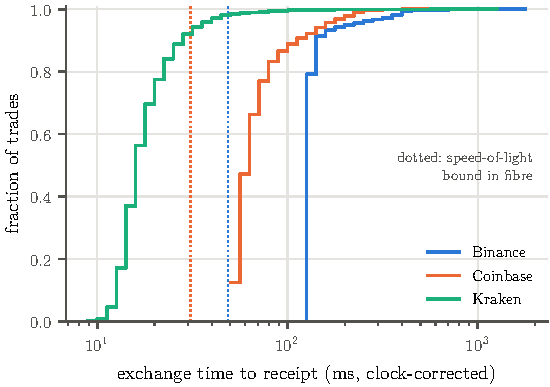
\includegraphics[width=0.62\textwidth]{figures/latency_cdf.pdf}
  \caption{Distribution of the corrected latency over the quiet baseline; dotted lines are the speed-of-light
  bounds in fibre.}
  \label{fig:latency-cdf}
\end{figure}

\begin{figure}[ht]
  \centering
  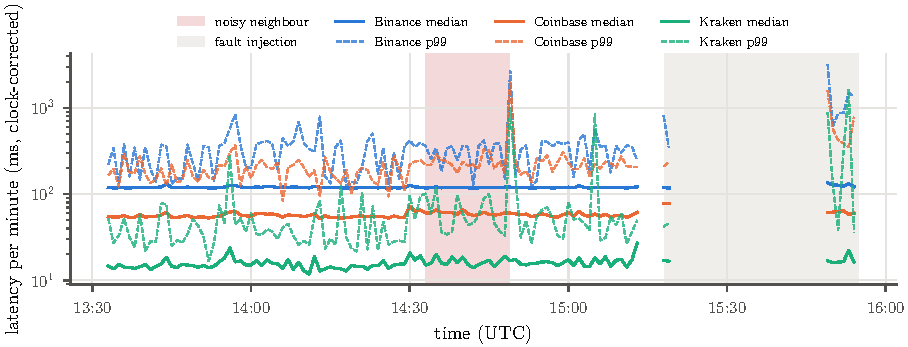
\includegraphics[width=\textwidth]{figures/latency_time.pdf}
  \caption{Median and 99th percentile of the corrected latency, per minute, over the whole experiment.}
  \label{fig:latency-time}
\end{figure}

The medians are stable to within a few milliseconds for two hours (\cref{fig:latency-time}), but the tails are long: the 99th
percentile is \LatBinancePninetynine\ms{} for Binance, \LatCoinbasePninetynine\ms{} for Coinbase and
\LatKrakenPninetynine\ms{} for Kraken, three to four times the median. They occur in bursts of trading, when a
venue publishes hundreds of messages within a few milliseconds.

\paragraph{Where the delay comes from.} Binance's event time $E$ separates its internal delay from transport:
the median of $E - T$ is \EminusTMedianMs\ms{} (maximum \EminusTMaxMs\ms), so Binance publishes trades almost as
soon as they happen and the tail arises between publication and receipt. To locate it, the independent probe
recorded the same quantity $t_{\mathrm{rx}} - E$ for BTC-USDT in a separate process (\cref{fig:probe}). The two
agree closely: over the \ProbeQuietSeconds{} seconds of the quiet baseline, the pipeline's per-second median
exceeds the probe's by \ProbeQuietDiffMedianMs\ms{} in the median, and most spikes appear in both series, which
places them upstream, in the network or in Binance's distribution layer. The tails differ, however: the
pipeline's excess reaches \ProbeQuietDiffPninetynineMs\ms{} at the 99th percentile, and it saw
\ProbeQuietPipeOverHalfSec{} seconds with a median above 500\ms{} against \ProbeQuietProbeOverHalfSec{} for
the probe.

The planned noisy-neighbour phase was meant to test whether this excess comes from competition for the CPU.
It does not: while the tests and the benchmark ran, the pipeline's excess over the probe was \emph{smaller}
(\ProbeNoisyDiffPninetynineMs\ms{} at the 99th percentile), its event-loop lag was unchanged
(\LoopLagNoisyPninetynine\ms{} at the 99th percentile, against \LoopLagQuietPninetynine\ms{} when quiet), and so
was its internal latency (\cref{tab:internal}). On a 16-thread machine, a load of this size leaves the pipeline
unaffected. The difference that remains between the two receivers is what they subscribe to: the probe receives
one trade stream, while the pipeline's Binance connection also carries two order book streams, which weigh far
more. During a burst, trades queue behind order book updates on the same TCP connection. The observations are
consistent with this head-of-line blocking, although the experiment does not isolate it; the design consequence
is that latency-critical streams belong on dedicated connections.

\begin{figure}[ht]
  \centering
  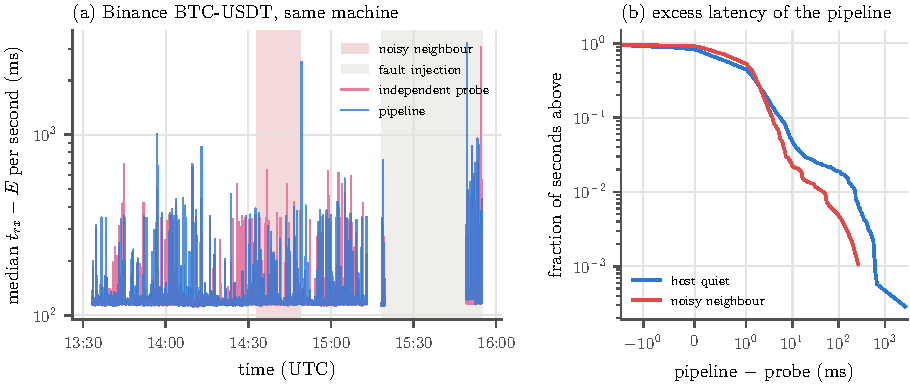
\includegraphics[width=\textwidth]{figures/probe.pdf}
  \caption{Control experiment. (a) Per-second median of $t_{\mathrm{rx}} - E$ for Binance BTC-USDT, measured by
  the pipeline and by an independent minimal receiver on the same machine. (b) Distribution of the pipeline's
  excess over the probe, per second, in the quiet baseline and during the noisy-neighbour phase.}
  \label{fig:probe}
\end{figure}

\subsection{Message loss and recovery}\label{sec:res-losses}

\Cref{tab:gaps} lists every gap. During the \BaselineMinutes{} minutes of the baseline no feed disconnected and
no sequence number was missed. The planned stop produced one restart gap per instrument, \RestartMissing{}
trades in total, all recovered at start-up.

During fault injection the pipeline was disconnected \ChaosDisconnects{} times, for a median of
\ChaosDowntimeMedianS{} seconds; each disconnection produced a gap whose size grows with the time disconnected
and with the venue's activity (\cref{fig:gaps}), and every gap was repaired. The most severe fault, however,
was not injected: at \SuspensionStart{} the host was suspended for \SuspensionMinutes{} minutes. Nothing was
logged during that interval although reconnections are retried at least every 30 seconds, so the process was
not running. On resumption, the feeds failed to connect for a few seconds until the network was back, then
reconnected and detected \SuspensionMissing{} missing trades, including a single gap of \LargestGap{} trades
on \LargestGapWhere. All of them were recovered from the venues' histories within three minutes.

Overall the pipeline detected \TotalMissing{} missing trades and recovered \TotalRecovered{}
(\RecoveredPctText). No gap was ever detected inside a connection, as expected over TCP. The median time from
detection to repair was \RepairMedianS{} seconds, of which one second is a deliberate wait that lets the REST
history catch up with the stream. On the order book side, \BookResyncs{} broken update chains, all after
reconnections, triggered a rebuild from a snapshot; none of the \QuotesStored{} best quotes stored was crossed.

\begin{table}[ht]
\centering
\caption{Sessions ended, gaps by cause, trades missed and recovered, and order book resyncs, per run and venue.}
\label{tab:gaps}
\small
% Generated by analysis/make_figures.py
\begin{tabular}{llrrrrrrr}
\toprule
Run & Venue & Disconn. & \multicolumn{3}{c}{Trade gaps} & Missed & Recovered & Book \\
\cmidrule(lr){4-6}
 & & & in session & reconnect & restart & trades & trades & resyncs \\
\midrule
baseline & Binance & 0 & 0 & 0 & 0 & 0 & 0 & 0 \\
 & Coinbase & 0 & 0 & 0 & 0 & 0 & 0 & 0 \\
 & Kraken & 0 & 0 & 0 & 0 & 0 & 0 & 0 \\
\midrule
chaos & Binance & 3 & 0 & 6 & 2 & 285\,964 & 285\,964 & 6 \\
 & Coinbase & 7 & 0 & 14 & 2 & 97\,344 & 97\,344 & 0 \\
 & Kraken & 4 & 0 & 8 & 2 & 8\,149 & 8\,149 & 0 \\
\bottomrule
\end{tabular}

\end{table}

\begin{figure}[ht]
  \centering
  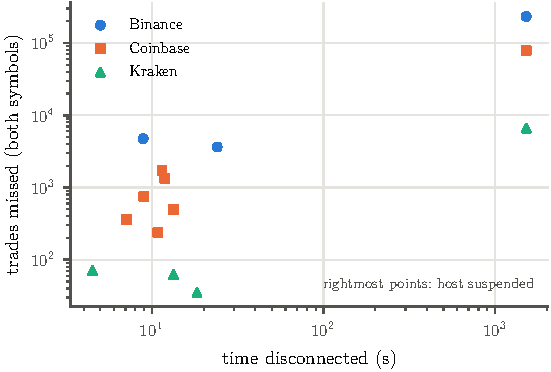
\includegraphics[width=0.62\textwidth]{figures/gaps_downtime.pdf}
  \caption{Fault-injection run: trades missed against the time disconnected, per venue. The rightmost points
  are the 26-minute host suspension.}
  \label{fig:gaps}
\end{figure}

The suspension also illustrates the difference between metrics and records. Prometheus ran in the same
suspended virtual machine and the counters restart with the process, so the dashboard's ``trades missed''
panel undercounts these events; the \code{gaps} table, written by the pipeline, has the exact count. Metrics are
for alerting; the database is the ledger.

\paragraph{Independent audit.} Sequence checks can only find what the pipeline knows to look for. The audit
compares every stored trade with the venue's own history for the same id range, per run and instrument
(\cref{tab:audit}). Out of \AuditReference{} trades in the venues' histories, \AuditMissing{} were missing from
the database, \AuditUnexpected{} were in the database but not in the history, and \AuditMismatched{} differed
in price, quantity, side or time; \AuditRecovered{} of the stored trades had been recovered by the backfill.

\begin{table}[ht]
\centering
\caption{Completeness audit against each venue's REST history (first and last minute of each run excluded).}
\label{tab:audit}
\small
% Generated by analysis/make_figures.py
\begin{tabular}{lllrrrrrr}
\toprule
Run & Venue & Symbol & Reference & Stored & Recovered & Missing & Extra & Altered \\
\midrule
baseline & Binance & BTC-USDT & 349\,886 & 349\,886 & 0 & 0 & 0 & 0 \\
 & Binance & ETH-USDT & 289\,343 & 289\,343 & 0 & 0 & 0 & 0 \\
 & Coinbase & BTC-USD & 164\,668 & 164\,668 & 0 & 0 & 0 & 0 \\
 & Coinbase & ETH-USD & 34\,583 & 34\,583 & 0 & 0 & 0 & 0 \\
 & Kraken & BTC-USD & 12\,326 & 12\,326 & 0 & 0 & 0 & 0 \\
 & Kraken & ETH-USD & 3\,777 & 3\,777 & 0 & 0 & 0 & 0 \\
\midrule
chaos & Binance & BTC-USDT & 135\,875 & 135\,875 & 122\,750 & 0 & 0 & 0 \\
 & Binance & ETH-USDT & 128\,998 & 128\,998 & 115\,423 & 0 & 0 & 0 \\
 & Coinbase & BTC-USD & 75\,432 & 75\,432 & 68\,030 & 0 & 0 & 0 \\
 & Coinbase & ETH-USD & 14\,046 & 14\,046 & 12\,839 & 0 & 0 & 0 \\
 & Kraken & BTC-USD & 5\,295 & 5\,295 & 4\,871 & 0 & 0 & 0 \\
 & Kraken & ETH-USD & 2\,073 & 2\,073 & 1\,865 & 0 & 0 & 0 \\
\bottomrule
\end{tabular}

\end{table}

\subsection{Pipeline internals and storage}

\Cref{tab:internal} gives the latencies inside the pipeline, on the monotonic clock. A trade reaches the
database \IngestQuietPfifty\ms{} after receipt in the median and \IngestQuietPninetynine\ms{} at the 99th
percentile, mostly the batching delay (a batch waits up to 100\ms{} for more rows) plus the write itself.
Decoding a Binance message takes about \ParseBinancePfiftyUs\,$\mu$s. The median event-loop lag of a few
milliseconds reflects the 15.6\ms{} timer resolution of Windows rather than load.

\begin{table}[ht]
\centering
\caption{Internal latencies (ms), from Prometheus histograms, per analysis window (the fault-injection window
excludes the suspension).}
\label{tab:internal}
\small
% Generated by analysis/make_figures.py
\begin{tabular}{lrrrrrr}
\toprule
Stage (ms) & \multicolumn{2}{c}{quiet baseline} & \multicolumn{2}{c}{noisy neighbour} & \multicolumn{2}{c}{fault injection} \\
\cmidrule(lr){2-3}\cmidrule(lr){4-5}\cmidrule(lr){6-7}
 & p50 & p99 & p50 & p99 & p50 & p99 \\
\midrule
Receipt to commit, trades & 125 & 318 & 126 & 298 & 132 & 422 \\
Receipt to commit, quotes & 104 & 262 & 107 & 274 & 114 & 337 \\
Batch write (COPY + insert) & 18.2 & 93.4 & 19.5 & 97.3 & 20.9 & 115 \\
Event loop lag & 6.49 & 24.2 & 5.78 & 24.1 & 6.43 & 24.7 \\
\bottomrule
\end{tabular}

\end{table}

The write path was benchmarked separately on 100\,000 synthetic trades (\cref{tab:storage}). The COPY-based
path is up to \BenchSpeedupMax{} times faster than \code{executemany} and reaches about \BenchBestRowsPerS{} rows
per second; replaying rows already stored is faster still, so idempotency costs little. The bottleneck is
index maintenance and continuous-aggregate invalidation on the hypertable; the deduplicating anti-join takes a
few milliseconds per batch. This capacity is about \CapacityRatio{} times the busiest minute observed
(\BusiestTradesPerS{} trades per second across all venues). Compressed, the
\TradesRows{} trades of the experiment occupy \TradesMBCompressed{} MB instead of \TradesMBUncompressed{} MB
(ratio \CompressionRatio), about \BytesPerTradeCompressed{} bytes per trade.

\begin{table}[ht]
\centering
\caption{Write throughput (rows per second) of the two insert strategies, on fresh rows and on a full replay
of rows already stored.}
\label{tab:storage}
\small
% Generated by analysis/make_figures.py
\begin{tabular}{rrrrr}
\toprule
Batch & \multicolumn{2}{c}{COPY + deduplicating insert} & \multicolumn{2}{c}{executemany} \\
\cmidrule(lr){2-3}\cmidrule(lr){4-5}
rows & new rows/s & replay rows/s & new rows/s & replay rows/s \\
\midrule
100 & 3\,976 & 7\,282 & 1\,480 & 1\,970 \\
1\,000 & 11\,646 & 16\,485 & 3\,720 & 3\,890 \\
10\,000 & 11\,092 & 93\,594 & 2\,990 & 3\,132 \\
\bottomrule
\end{tabular}

\end{table}


% =====================================================================================================
\section{Limitations}\label{sec:limitations}

\begin{itemize}[nosep]
  \item \emph{Clock assumptions.} The correction assumes the venues' clocks are synchronised to UTC; it removes
        our clock error, not theirs. One-way latencies remain uncertain by the NTP error bound.
  \item \emph{Measurement point.} Receipt is timestamped in user space after the TLS and websocket layers.
        Kernel or NIC timestamps would remove the event-loop component, and on Windows the event loop's timer
        resolution (15.6\ms) inflates the measured loop lag.
  \item \emph{Network.} The experiment ran over a university Wi-Fi network, whose latency and loss are not
        those of a co-located or even a wired connection; the absolute latencies are specific to that setup.
  \item \emph{Metrics during outages.} Prometheus counters restart with the process and miss what happens while
        the host is down, so dashboards undercount losses around restarts; the \code{gaps} table is the record.
  \item \emph{Single process, single host.} The pipeline is not highly available: a host failure is recovered
        from the REST history at restart, within the venues' history and rate limits. A production system would
        run redundant ingestors in different regions, behind a log such as Kafka \citep{kreps2011,kleppmann2017}.
  \item \emph{Order books.} Order book losses are detected and resynchronised but cannot be backfilled, and the
        local book is only checked for internal consistency (it must never be crossed).
\end{itemize}

\section{Conclusion}

The pipeline turns two usually implicit properties of market data, completeness and timeliness, into measured
quantities. Sequence numbers make losses exact; the venues' histories and idempotent storage make them
recoverable; an independent audit confirms the result. Latencies are corrected for the local clock, bounded by
physics, and separated from the pipeline's own delay by a control experiment. The same principles carry over to
professional feeds, where sequence numbers, gap-fill services and hardware timestamps play the roles of the
public APIs used here.

\appendix
\section{Reproducing the results}

\begin{verbatim}
docker compose up -d                     # TimescaleDB, Prometheus, Grafana
pip install -e ".[dev,analysis]"
marketpipe run --label baseline --duration 6000   # then a 5-minute stop
marketpipe run --label chaos --chaos --chaos-interval 120 --duration 2700
python tools/latency_probe.py            # in parallel: the control experiment
python analysis/export.py --audit --compress      # -> results/*.csv
python analysis/make_figures.py          # figures, tables, macros
\end{verbatim}

\bibliographystyle{plainnat}
\bibliography{references}

\end{document}
